\documentclass[12pt]{article}
\usepackage[left=1cm, right=1cm, top=2cm,bottom=1.5cm]{geometry} 

\usepackage[parfill]{parskip}
\usepackage[utf8]{inputenc}
\usepackage[T2A]{fontenc}
\usepackage[russian]{babel}
\usepackage{enumitem}
\usepackage[normalem]{ulem}
\usepackage{amsfonts, amsmath, amsthm, amssymb, mathtools}

\usepackage{tabularx}
\usepackage{hhline}

\usepackage{accents}
\usepackage{fancyhdr}
\pagestyle{fancy}
\renewcommand{\headrulewidth}{1.5pt}
\renewcommand{\footrulewidth}{1pt}

\usepackage{graphicx}
\usepackage[figurename=Рис.]{caption}
\usepackage{subcaption}
\usepackage{float}

%%Наименование папки откуда забирать изображения
\graphicspath{ {./images/} }

%%Изменение формата для ввода доказательства
\renewcommand{\proofname}{$\square$  \nopunct}
\renewcommand\qedsymbol{$\blacksquare$}

%%Изменение отступа на таблицах
\addto\captionsrussian{%
	\renewcommand{\proofname}{$\square$ \nopunct}%
}
%% Римские цифры
\newcommand{\RN}[1]{%
	\textup{\uppercase\expandafter{\romannumeral#1}}%
}

%% Для удобства записи
\newcommand{\MR}{\mathbb{R}}
\newcommand{\MC}{\mathbb{C}}
\newcommand{\MQ}{\mathbb{Q}}
\newcommand{\MN}{\mathbb{N}}
\newcommand{\MZ}{\mathbb{Z}}
\newcommand{\MTB}{\mathbb{T}}
\newcommand{\MTI}{\mathbb{I}}
\newcommand{\MI}{\mathrm{I}}
\newcommand{\MJ}{\mathrm{J}}
\newcommand{\MH}{\mathrm{H}}
\newcommand{\MT}{\mathrm{T}}
\newcommand{\MU}{\mathcal{U}}
\newcommand{\MV}{\mathcal{V}}
\newcommand{\MB}{\mathcal{B}}
\newcommand{\MW}{\mathcal{W}}
\newcommand{\ML}{\mathcal{L}}
\newcommand{\MP}{\mathcal{P}}
\newcommand{\VN}{\varnothing}
\newcommand{\VE}{\varepsilon}

\theoremstyle{definition}
\newtheorem{defn}{Опр:}
\newtheorem{rem}{Rm:}
\newtheorem{prop}{Утв.}
\newtheorem{exrc}{Упр.}
\newtheorem{lemma}{Лемма}
\newtheorem{theorem}{Теорема}
\newtheorem{corollary}{Следствие}

\newenvironment{cusdefn}[1]
{\renewcommand\thedefn{#1}\defn}
{\enddefn}

\DeclareRobustCommand{\divby}{%
	\mathrel{\text{\vbox{\baselineskip.65ex\lineskiplimit0pt\hbox{.}\hbox{.}\hbox{.}}}}%
}
%Короткий минус
\DeclareMathSymbol{\SMN}{\mathbin}{AMSa}{"39}
%Длинная шапка
\newcommand{\overbar}[1]{\mkern 1.5mu\overline{\mkern-1.5mu#1\mkern-1.5mu}\mkern 1.5mu}
%Функция знака
\DeclareMathOperator{\sgn}{sgn}

%Функция ранга
\DeclareMathOperator{\rk}{\text{rk}}

%Обозначение константы
\DeclareMathOperator{\const}{\text{const}}

\DeclareMathOperator*{\dsum}{\displaystyle\sum}
\newcommand{\ddsum}[2]{\displaystyle\sum\limits_{#1}^{#2}}

%Интеграл в большом формате
\DeclareMathOperator{\dint}{\displaystyle\int}
\newcommand{\ddint}[2]{\displaystyle\int\limits_{#1}^{#2}}
\newcommand{\ssum}[1]{\displaystyle \sum\limits_{n=1}^{\infty}{#1}_n}

\newcommand{\smallerrel}[1]{\mathrel{\mathpalette\smallerrelaux{#1}}}
\newcommand{\smallerrelaux}[2]{\raisebox{.1ex}{\scalebox{.75}{$#1#2$}}}

\newcommand{\smallin}{\smallerrel{\in}}
\newcommand{\smallnotin}{\smallerrel{\notin}}

\newcommand*{\medcap}{\mathbin{\scalebox{1.25}{\ensuremath{\cap}}}}%
\newcommand*{\medcup}{\mathbin{\scalebox{1.25}{\ensuremath{\cup}}}}%

\makeatletter
\newcommand{\vast}{\bBigg@{3.5}}
\newcommand{\Vast}{\bBigg@{5}}
\makeatother

%Промежуточное значение для sup\inf, поскольку они имеют разную высоту
\newcommand{\newsup}{\mathop{\smash{\mathrm{sup}}}}
\newcommand{\newinf}{\mathop{\mathrm{inf}\vphantom{\mathrm{sup}}}}

%Скалярное произведение
\newcommand{\inner}[2]{\left\langle #1, #2 \right\rangle }

%Подпись символов снизу
\newcommand{\ubar}[1]{\underaccent{\bar}{#1}}

%% Шапка для букв сверху
\newcommand{\wte}[1]{\widetilde{#1}}

%%Функция для обозначения равномерной сходимости по множеству
\newcommand{\uconv}[1]{\overset{#1}{\rightrightarrows}}
\newcommand{\uconvm}[2]{\overset{#1}{\underset{#2}{\rightrightarrows}}}


%%Функция для обозначения нижнего и верхнего интегралов
\def\upint{\mathchoice%
	{\mkern13mu\overline{\vphantom{\intop}\mkern7mu}\mkern-20mu}%
	{\mkern7mu\overline{\vphantom{\intop}\mkern7mu}\mkern-14mu}%
	{\mkern7mu\overline{\vphantom{\intop}\mkern7mu}\mkern-14mu}%
	{\mkern7mu\overline{\vphantom{\intop}\mkern7mu}\mkern-14mu}%
	\int}
\def\lowint{\mkern3mu\underline{\vphantom{\intop}\mkern7mu}\mkern-10mu\int}


\begin{document}
\lhead{Математический анализ - \RN{3}}
\chead{Шапошников С.В.}
\rhead{Лекция - 27}
\section*{Ряды Фурье}
\subsection*{Мотивация для рядов Фурье}
Рассмотрим пространство $\MR^3$, в нём есть скалярное произведение $\inner{x}{y} = x_1 y_1 + x_2 y_2 + x_3 y_3$. Пусть в $\MR^3$ также задан ортонормированный базис:
$$
	\begin{array}{rcl}
		e_1 &=& (1,0,0)\\
		e_2 &=& (0,1,0) \\
		e_3 &=& (0,0,1)
	\end{array} \text{ - о.н.с.}, \, 
	\inner{e_i}{e_j} = 
	\left\{
		\begin{array}{rl}
			1, & i = j\\
			0, & i \neq j
		\end{array}
	\right., \, \forall i, \, \|e_i\| = 1
$$
Длину определяем как и раньше: $\|x\| = \sqrt{\inner{x}{x}}$. Оказывается, что:
$$
	\forall x \in \MR^3, \, x = x_1 e_1 + x_2 e_2 + x_3 e_3
$$
Это называется рядом Фурье, где $x_i$ можно находить так: $x_i = \inner{x}{e_i}$ - коэффициенты Фурье. Одновременно с этим, верна теорема Пифагора:
$$
	\|x\|^2 = |x_1|^2 + |x_2|^2 + |x_3|^2
$$
это равенство будут называть равенством Парсеваля или равенством Ляпунова (модули стоят, чтобы индексы не потерялись). Также заметим, что если взять не все $e_j$, а только два из них или один, или ничего, то не всякий $x$ разложиться в ряд Фурье. Нужна полнота.
\subsection*{Евклидово пространство}
\begin{defn}
	Пусть $E$ - линейное пространство над $\MC$ (или $\MR$). Предположим, что на $E\times E$ определена функция со значениями в $\MC$ (или в $\MR$), удовлетворяющая следующими свойствами:
	\begin{enumerate}[label=\arabic*)]
		\item $\inner{x}{x}\in\MR, \, \inner{x}{x} \geq 0, \, \inner{x}{x} = 0 \Leftrightarrow x = 0$;
		\item $\inner{x}{y} = \overline{\inner{y}{x}}$;
		\item $\inner{\alpha x_1 + \beta x_2}{y} =  \alpha \inner{x_1}{y} + \beta \inner{x_2}{y}$;
	\end{enumerate}
	Тогда $\inner{\cdot}{\cdot}$ называется \uwave{скалярным произведением}, а $E$ называют \uwave{Евклидовым пространством}.
\end{defn}
\begin{rem}
	В линейной алгебре пространства над $\MC$ описанное выше называют обычно \uwave{Эрмитовым}, тогда как в анализе обычно делят пространства на Евклидовы и \uwave{Гильбертовы}, где в Евклидовом не требуется никакой полноты, а в Гильбертовом требуется полнота.
\end{rem}

\begin{defn}
	\uwave{Нормой} будем называть корень из скалярного произведения: $\|x\| = \sqrt{\inner{x}{x}}$.
\end{defn}

\begin{theorem}(\textbf{неравенство Коши-Буняковского-Шварца})
	$$
		\forall x,y, \, |\inner{x}{y}| \leq \|x\|{\cdot}\|y\|
	$$
\end{theorem}
\begin{proof}
	Рассмотрим квадратный трехчлен, пусть $t \in \MR$, тогда:
	$$
		0\leq \inner{x -ty}{x-ty} = \|x\|^2 - t\inner{y}{x} - t\inner{x}{y} + t^2\|y\|^2 = \|x\|^2 - 2t\operatorname{Re}\inner{x}{y} + t^2\|y\|^2
	$$
	где последнее равенство верно в силу: $z + \overline{z} = a + bi + a - bi = 2a = 2\operatorname{Re}z$. Теперь возможны две ситуации:
	\begin{enumerate}[label=(\arabic*)]
		\item Пусть $\|y\| =0 \Rightarrow y = 0 \Rightarrow 0 \leq 0$ - выполнено;
		\item Пусть $\|y\| \neq 0 \Rightarrow D \leq 0 \Leftrightarrow 4(\operatorname{Re}\inner{x}{y})^2 - 4\|x\|^2{\cdot}\|y\|^2 \leq 0 \Leftrightarrow |\operatorname{Re}\inner{x}{y}| \leq \|x\|{\cdot}\|y\|$, поскольку полученное неравенство справедливо для любых $x,y$, то возьмем $x = \lambda z, \, \lambda \in \MC$, тогда:
		$$
			\forall y,z, \, \forall \lambda \in \MC,\, |\operatorname{Re}\lambda\inner{z}{y}| \leq |\lambda|{\cdot}\|z\|{\cdot}\|y\|
		$$
		Пусть $|\lambda| = 1 \Rightarrow$ мы получим неравенство: 
		$$
			\forall y,z, \, \forall \lambda \in \MC,\,|\lambda|=1 ,\, |\operatorname{Re}\lambda\inner{z}{y}| \leq \|z\|{\cdot}\|y\|
		$$ 
		Умножение на комплексное число, по модулю равное единице, это поворот:
		$$
			z = x + iy \Rightarrow z = re^{i\theta}, \, |z| = 1 \Rightarrow  |z| = r = 1 \Rightarrow z = e^{i\theta} = \cos{\theta} + i\sin{\theta} \Rightarrow z{\cdot}\overline{z} = e^{i\theta}e^{-i\theta} = 1 = |z|
		$$
		\begin{figure}[H]
			\centering
			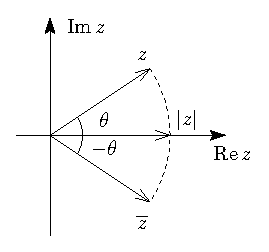
\includegraphics[width=0.25\textwidth]{MA3L27_1.eps}
			\label{MA3L27_1}
			\caption{Поворот на плоскости через домножение комплексного числа.}
			\label{fig: Поворот на плоскости}
		\end{figure}
		Следовательно, мы можем выбрать $\lambda$ так, чтобы повернуть $\lambda \inner{z}{y}$ до его модуля: $\lambda \inner{z}{y} = |\inner{z}{y}|$. 
		Это $\lambda$ можно выбрать явно:
		$$
			\lambda = \dfrac{\overline{\inner{z}{y}}}{|\inner{z}{y}|} \Rightarrow \lambda\inner{z}{y} = \dfrac{\inner{z}{y}{\cdot}\overline{\inner{z}{y}}}{|\inner{z}{y}|} = \dfrac{|\inner{z}{y}|^2}{|\inner{z}{y}|} = |\inner{z}{y}| \Rightarrow |\operatorname{Re}\lambda\inner{z}{y}| = |\inner{z}{y}|\leq \|z\|{\cdot}\|y\|
		$$
		Отметим, что в случае вещественного $\inner{x}{y}$ равенство равносильно $D = 0 \Rightarrow$ есть корень в уравнении: $\inner{x -ty}{x-ty} = 0 \Rightarrow \exists \, t \colon \inner{x - ty}{x - ty} = 0 \Rightarrow x = ty$, то есть получили линейную зависимость. В случае, если $\inner{x}{y}$ не вещественно, то удобно перевести в вещественный случай $\Rightarrow$ представим $x$ в виде: $x = \lambda z \Rightarrow \exists \, \lambda \colon \inner{x}{y} =  \inner{\lambda z}{y}  =\lambda \inner{z}{y	} \in \MR \Rightarrow \exists \, t \colon \lambda z - ty = 0 \Rightarrow \lambda z =ty$, следовательно опять получили линейную зависимость. 
	\end{enumerate}
\end{proof}

\begin{corollary}
	Норма $\|x\|$ - это действительно норма, то есть:
	\begin{enumerate}[label=\arabic*)]
		\item $\|x\| \geq 0, \, \|x\| = 0 \Leftrightarrow x = 0$;
		\item $\|\alpha x\| = |\alpha|{\cdot}\|x\|$;
		\item $\|x + y\| \leq \|x\| + \|y\|$;
	\end{enumerate} 
\end{corollary}
\begin{proof}Свойства $1)-2)$ следуют сразу из свойств скалярного произведения:
	\begin{enumerate}[label=\arabic*)]
		\item $\|x\| = \sqrt{\inner{x}{x}} \geq 0, \, \|x\| =  \sqrt{\inner{x}{x}} = 0 \Leftrightarrow x = 0$;
		\item $\|\alpha x\| = \sqrt{\inner{\alpha x}{\alpha x}} =\sqrt{\alpha\overline{\inner{\alpha x}{x}}} = \sqrt{\alpha{\cdot}\overline{\alpha}\inner{x}{x}} = \sqrt{|\alpha|^2  \inner{x}{x}} = |\alpha|{\cdot}\|x\|$;
		\item Распишем квадрат нормы от $x+y$:
		$$
			\|x + y\|^2  = \inner{x+y}{x+y} = \|x\|^2 + 2\operatorname{Re}\inner{x}{y} + \|y\|^2
		$$ 
		Поскольку верно: $\operatorname{Re}z = \operatorname{Re}(x + iy) = x \leq |z| = \sqrt{x^2 + y^2}$, то воспользуемся этим и применим неравенство КБШ:
		$$
			\|x + y\|^2 \leq \|x\|^2 + 2|\inner{x}{y}| +  \|y\|^2 \leq \|x\|^2 + 2\|x\|{\cdot}\|y\|+  \|y\|^2 = (\|x\| + \|y\|)^2
		$$
		Берем корень и за счет неотрицательности получаем требуемое;
	\end{enumerate} 
\end{proof}
\begin{prop}
	Равенство параллелограмма: $\|x + y\|^2 + \|x - y\|^2 = 2\|x\|^2 + 2\|y\|^2$.
\end{prop}
\begin{proof}
	По определению:
	$$
		\|x+y\|^2 =\inner{x+y}{x+y} = \inner{x}{x} + \inner{x}{y} + \inner{y}{x} + \inner{y}{y} = \|x\|^2 + 2\operatorname{Re}\inner{x}{y} + \|y\|^2
	$$
	$$
		\|x-y\|^2 =\inner{x-y}{x-y} = \inner{x}{x} - \inner{x}{y} - \inner{y}{x} + \inner{y}{y} = \|x\|^2 - 2\operatorname{Re}\inner{x}{y} + \|y\|^2
	$$
	Складываем два равенства и получаем требуемое.
\end{proof}
\begin{rem}
	Отметим, что если равенство параллелограмма выполнено, то норма задается скалярным произведением. Если дали норму и пообещали, что она относится к скалярному произведению, то её легко восстановить. Например, в случае $\MR$ будет верно: 
	$$
		\|x + y\|^2 = \|x\|^2 + 2\inner{x}{y} + \|y\|^2
	$$ 
	тогда скалярное произведение будет иметь следующий вид:
	$$
		\inner{x}{y} = \dfrac{1}{2}\left(\|x + y\|^2 - \|x\|^2 - \|y\|^2 \right)
	$$
	Из линейной алгебры: билинейная форма восстанавливается по квадратичной функции. Остается вопрос, будут ли выполнены свойства скалярного произведения? Можно показать, что равенства параллелограмма достаточно, чтобы это оказалось скалярным произведением и свойства выполнялись.
\end{rem}
\begin{exrc}
	Проверить, что на $\MR^2$ норма вида: $\|x\| = |x_1| + |x_2|$ не является нормой, порожденной скалярным произведением.
\end{exrc}

\newpage
\subsection*{Сходимость в Евклидовых пространствах}
Мы получили нормированное пространство $(E, \|\cdot\|)$. Значит можем определить в нём сходимости.
\begin{defn}
	Последовательность $\{x_n\}$ \uwave{сходится} к $x$ в нормированном пространстве $(E,\|\cdot\|)$, тогда и только тогда, когда: 
	$$
		x = \lim\limits_{n \to \infty}x_n \Leftrightarrow \|x_n - x\| \to 0
	$$
\end{defn}
\begin{defn}
	Ряд $\ddsum{n = 1}{\infty}x_k$ \uwave{сходится} к $x$ в нормированном пространстве $(E,\|\cdot\|)$, тогда и только тогда, когда: 
	$$
		x = \lim\limits_{N \to \infty}\ddsum{k = 1}{N}x_k \Leftrightarrow \left\|\ddsum{k = 1}{N}x_k - x\right\| \to 0
	$$
\end{defn}

\begin{corollary}
	Если $x_n \to x$ и $y_n \to y$, то $\inner{x_n}{y_n} \to \inner{x}{y}$, то есть скалярное произведение непрерывно по совокупности переменных.
\end{corollary}
\begin{proof}
	Рассмотрим разность:
	$$
		|\inner{x}{y} - \inner{x_n}{y_n}| \leq |\inner{x}{y} - \inner{x_n}{y}| + |\inner{x_n}{y} - \inner{x_n}{y_n}| = |\inner{x - x_n}{y}| + |\inner{x_n}{y - y_n}|
	$$
	Воспользуемся неравенством КБШ:
	$$
		|\inner{x - x_n}{y}| + |\inner{x_n}{y - y_n}| \leq \|x - x_n\|{\cdot}\|y\| + \|x_n\|{\cdot}\|y - y_n\| \leq \|x - x_n\|{\cdot}\|y\| + C{\cdot}\|y - y_n\| \to 0
	$$
	где в последнем неравенстве мы воспользовались ограниченностью $x_n$, так как она сходится.
\end{proof}

\subsection*{Примеры Евклидовых пространств}

\begin{enumerate}[label=\arabic*)]
	\item $E = \MR^n, \, \inner{x}{y} = \ddsum{k = 1}{n}x_k y_k$
	\begin{proof}
		Проверялось во $2$-ом семестре;
	\end{proof}
	\item $E = \MC^n, \, \inner{x}{y} = \ddsum{k = 1}{n}x_k \overline{y}_k$
	\begin{proof}
		Проверяется на линейной алгебре;
	\end{proof} 
	\item $E = R[a,b]$ - интегрируемые по Риману функции на $[a,b]$, $\inner{f}{g} = \ddint{a}{b}f(t)\overline{g(t)}dt$;
	\begin{proof}
		Проверим, будет ли указанный объект скалярным произведением:
		\begin{enumerate}[label=\arabic*)]
			\item Рассмотрим $\inner{f}{f}$:
			$$
				\inner{f}{f} = \ddint{a}{b}|f(t)|^2dt \geq 0, \, \ddint{a}{b}|f(t)|^2dt = 0 \Leftarrow f = 0
			$$
			Обратное для последнего - не выполняется, но мы получим, что $f$ почти всюду $0$: 
			$$
				\ddint{a}{b}|f(t)|^2dt = 0 \Rightarrow f \overset{\text{п.в.}}{=} 0
			$$
			Введём на $R[a,b]$ отношения эквивалентности: 
			$$
				f \sim g \Leftrightarrow f \overset{\text{п.в.}}{=} g
			$$ 
			Далее, под $R[a,b]$ будем понимать множество классов эквивалентности и будем отождествлять функции, которые отличаются на множестве меры ноль. В этом случае $1)$ будет выполнятся;
			\item Очевидно:
			$$
				\inner{f}{g} = \ddint{a}{b}f(t)\overline{g(t)}dt = \ddint{a}{b}\overline{g(t) \overline{f(t)}}dt = \overline{\inner{g}{f}}
			$$
			\item Очевидно из линейности интеграла: 
			$$
				\inner{\alpha f_1 + \beta f_2}{g} = \ddint{a}{b}(\alpha f_1(t) + \beta f_2(t))\overline{g(t)}dt = \alpha \ddint{a}{b}f_1(t)\overline{g(t)}dt + \beta \ddint{a}{b}f_2(t)\overline{g(t)}dt =
			$$
			$$
				 = \alpha\inner{f_1}{g} + \beta\inner{f_2}{g}
			$$
		\end{enumerate}
	\end{proof}
\end{enumerate}

\begin{defn}
	В линейном пространстве $E$ будем говорить, что вектор $u$ \uwave{ортогонален} вектору $v$, если: 
	$$
		\forall u,v \in E, \, u \bot v \Leftrightarrow \inner{u}{v} = 0
	$$
\end{defn}
\begin{rem}
	Заметим, что нулевой вектор ортогонален всем векторам: $\inner{0}{v} = 0, \, \forall v \in E$.
\end{rem}
\begin{theorem}(\textbf{Пифагора})
	\begin{enumerate}[label=(\arabic*)]
		\item Если $u\bot v$, то $\|u + v\|^2 = \|u\|^2 + \|v\|^2$;
		\item Если $u = \ddsum{n}{}u_n$ и $\forall n \neq m, \, u_n \bot u_m$, то $\|u\|^2 = \ddsum{n}{}\|u_n\|^2$;
	\end{enumerate}
\end{theorem}
\begin{rem}
	Заметим, что в отличии от школьной теоермы обратные равенства не верны:
	$$
		\|u\|^2 + 2\operatorname{Re}\inner{u}{v} + \|v\|^2 = \|u + v\|^2 = \|u\|^2 + \|v\|^2 \Rightarrow 2\operatorname{Re}\inner{u}{v} = 0
	$$
	Таким образом, теорема будет верна в обратную сторону только в вещественном случае, но в комплексном случае будет верна только в одну сторону.
\end{rem}
\begin{proof}\hfill
	\begin{enumerate}[label=(\arabic*)]
		\item По определению нормы: $\|u + v\|^2  = \|u\|^2 + 2\operatorname{Re}\inner{x}{y} + \|v\|^2 = \|u\|^2 + \|v\|^2$;
		\item Следует сразу из предыдущего пункта по индукции для конечного случая. Для бесконечного случая применяется конечный и берется предел;
	\end{enumerate}
\end{proof}

\newpage
\subsection*{Ортонормированные системы}
\begin{defn}
	Конечный или счётный набор векторов $\{e_k\}$ называется \uwave{ортонормированной системой} (о.н.с.), если выполняются следующие условия:
	\begin{enumerate}[label=(\arabic*)]
		\item $\forall k, \, \|e_k\| = 1$;
		\item $ \forall k \neq m, \, e_k \bot e_m, \, \Leftrightarrow  \forall k \neq m, \, \inner{e_k}{e_m} = 0$
	\end{enumerate}
\end{defn}
\begin{defn}
	$\forall x \in E$, числа $\hat{x}_k = \inner{x}{e_k}$ называются \uwave{коэффициентами Фурье}. 
\end{defn}
\begin{defn}
	Сумму вида $\ddsum{k}{}\hat{x}_ke_k$ называют \uwave{рядом Фурье} по системе $\{e_k\}$.
\end{defn}
Смысл коэффициентов Фурье состоит в проекции на $e_k$: $\hat{x}_k e_k$ - проекция на $e_k$, $\hat{x}_k$ - длина проекции. Смысл ряда Фурье: $x$ собирается как сумма своих проекций.

\begin{prop}
	Пусть $\MP = \langle e_1, \dotsc, e_N \rangle$ - линейная оболочка $e_1, \dotsc, e_N$, где $\{e_i\}_{i =1}^{N}$ - о.н.с., тогда:
	$$
		\forall x \in E, \, \forall y \in \MP, \, x - (\hat{x}_1 e_1 + \dotsc + \hat{x}_N e_N) \bot y
	$$
\end{prop}
\begin{rem}
	В линейной алгебре вектор разности выше принято называть \uwave{ортогональной проекцией} вектора $x$ на пространство $\MP$.
\end{rem}
\begin{figure}[H]
	\centering
	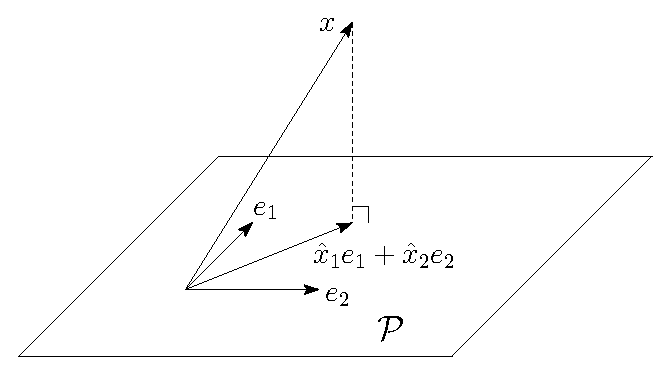
\includegraphics[width=0.5\textwidth]{MA3L27_2.eps}
	\label{MA3L27_2}
	\caption{Ортогональная проекция вектора $x$ на пространство $\MP$.}
	\label{fig: Проекция на пространство}
\end{figure}
\begin{proof}
	Поскольку $y \in \MP \Rightarrow y = c_1 e_1 + \dotsc + c_N e_N$, то достаточно проверить, что: 
	$$
		x - (\hat{x}_1 e_1 + \dotsc + \hat{x}_N e_N) \bot e_k, \, \forall k = \overline{1,N}
	$$
	Проверим ортогональность прямо по определению:
	$$
		\inner{x - (\hat{x}_1 e_1 + \dotsc + \hat{x}_N e_N)}{e_k} = \inner{x}{e_k} - \ddsum{j = 1}{N}\hat{x}_j\inner{e_j}{e_k} = \inner{x}{e_k} - \hat{x}_k\inner{e_k}{e_k} = \hat{x}_k - \hat{x}_k = 0
	$$
\end{proof}

\begin{prop}(\textbf{экстремальное свойство коэффициентов Фурье}) 
	Пусть $\MP = \langle e_1, \dotsc, e_N \rangle$ - линейная оболочка $e_1, \dotsc, e_N$, где $\{e_i\}_{i =1}^{N}$ - о.н.с., тогда:
	$$
		\forall x \in E, \, \min\limits_{y \in \MP}{\|x - y\|} = \left\|x - (\hat{x}_1 e_1 + \dotsc + \hat{x}_N e_N)\right\|
	$$
	и более того, $y = \hat{x}_1 e_1 + \dotsc + \hat{x}_N e_N \in \MP$ - единственный вектор на котором достигается минимум.
\end{prop}
\begin{figure}[H]
	\centering
	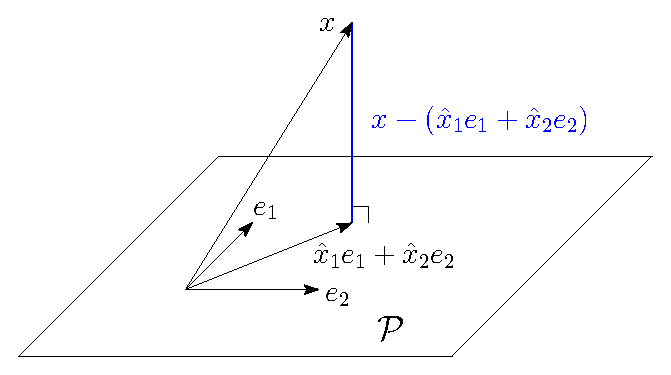
\includegraphics[width=0.5\textwidth]{MA3L27_3.eps}
	\label{MA3L27_3}
	\caption{Кратчайшее расстояние до $\MP$.}
	\label{fig: Кратчайшее расстояние}
\end{figure}
\begin{rem}
	Отметим, что идейно это метод наименьших квадратов (МНК): надо найти в линейной оболочке данных векторов ближайший к вектору $x$, тогда можно провести ортогонализацию этих векторов и ответ получим прямо по формуле в свойстве.
\end{rem}
\begin{proof}
	Пусть $y \in \MP$, рассмотрим квадрат расстояния: $\|x - y\|^2$, добавим и вычтем проекцию $x$ на $\MP$:
	$$
		\|x - y\|^2 = \left\|x - (\hat{x}_1 e_1 + \dotsc + \hat{x}_N e_N) + (\hat{x}_1 e_1 + \dotsc + \hat{x}_N e_N) - y\right\|^2
	$$
	$$
		x - (\hat{x}_1 e_1 + \dotsc + \hat{x}_N e_N) \bot \MP, \, (\hat{x}_1 e_1 + \dotsc + \hat{x}_N e_N) - y \in \MP \Rightarrow 
	$$
	$$
		\Rightarrow x - (\hat{x}_1 e_1 + \dotsc + \hat{x}_N e_N) \bot (\hat{x}_1 e_1 + \dotsc + \hat{x}_N e_N) - y
	$$
	Следовательно, мы можем применить теорему Пифагора:
	$$
		\|x - y\|^2 = \left\|x - (\hat{x}_1 e_1 + \dotsc + \hat{x}_N e_N)\right\|^2 + \left\| (\hat{x}_1 e_1 + \dotsc + \hat{x}_N e_N) - y\right\|^2 \geq \left\|x - (\hat{x}_1 e_1 + \dotsc + \hat{x}_N e_N)\right\|^2
	$$
	$$
		\left\| (\hat{x}_1 e_1 + \dotsc + \hat{x}_N e_N) - y\right\|^2\geq 0 \wedge \left\| (\hat{x}_1 e_1 + \dotsc + \hat{x}_N e_N) - y\right\|^2 = 0 \Leftrightarrow y = \hat{x}_1 e_1 + \dotsc + \hat{x}_N e_N \Rightarrow
	$$
	$$
		\Rightarrow \|x - y\|^2  = \left\|x - (\hat{x}_1 e_1 + \dotsc + \hat{x}_N e_N)\right\|^2 \Leftrightarrow y = \hat{x}_1 e_1 + \dotsc + \hat{x}_N e_N
	$$
\end{proof}

\begin{corollary}(\textbf{теорема Пифагора}) 
	Если $e_1, \dotsc, e_N$ - о.н.с., то верно следующее:
	$$
		\forall x \in E, \, \left\|x - \ddsum{k = 1}{N}\hat{x}_k e_k \right\|^2 = \|x\|^2 - \ddsum{k = 1}{N}\left|\hat{x}\right|^2
	$$
\end{corollary}
\begin{proof}
	Чтобы увидеть здесь теорему Пифагора, перенесем слагаемое с минусом в левую часть, тогда:
	$$
		\left\|x - \ddsum{k = 1}{N}\hat{x}_k e_k \right\|^2 + \ddsum{k = 1}{N}\left|\hat{x}\right|^2 = \|x\|^2
	$$	
	Одновременно с этим заметим:
	$$
		\|x\|^2 = \left\|x - \ddsum{k = 1}{N}\hat{x}_k e_k + \ddsum{k = 1}{N}\hat{x}_k e_k\right\|^2
	$$
	Выше мы доказали, что: $x - \ddsum{k = 1}{N}\hat{x}_k e_k \bot \ddsum{k = 1}{N}\hat{x}_k e_k$, тогда по теореме Пифагора:
	$$
		\left\|x - \ddsum{k = 1}{N}\hat{x}_k e_k + \ddsum{k = 1}{N}\hat{x}_k e_k\right\|^2 = \left\|x - \ddsum{k = 1}{N}\hat{x}_k e_k\right\|^2 + \left\|\ddsum{k = 1}{N}\hat{x}_k e_k\right\|^2 = \left\|x - \ddsum{k = 1}{N}\hat{x}_k e_k\right\|^2 + \ddsum{k = 1}{N}\left|\hat{x}_k\right|^2\|e_k\|^2 =
	$$
	$$
		=	\left\|x - \ddsum{k = 1}{N}\hat{x}_k e_k\right\|^2 + \ddsum{k = 1}{N}\left|\hat{x}_k\right|^2 \Rightarrow \|x\|^2 = \left\|x - \ddsum{k = 1}{N}\hat{x}_k e_k\right\|^2 + \ddsum{k = 1}{N}\left|\hat{x}_k\right|^2
	$$
\end{proof}
\begin{corollary}(\textbf{неравенство Бесселя})
	Если $\{e_k\}$ - конечная или счётная о.н.с., то верно следующее:
	$$
		\forall x \in E, \, \ddsum{k}{}|\hat{x}_k|^2 \leq \|x\|^2
	$$
\end{corollary}
\begin{proof}
	Используя предыдущее следствие, будет верно:
	$$
		\forall N \in \MN, \, \ddsum{k = 1}{N}\left|\hat{x}_k\right|^2 + \left\|x - \ddsum{k = 1}{N}\hat{x}_k e_k \right\|^2 = \|x\|^2, \, 0 \leq \left\|x - \ddsum{k = 1}{N}\hat{x}_k e_k \right\|^2  \Rightarrow \ddsum{k = 1}{N}\left|\hat{x}_k\right|^2  \leq \|x\|^2
	$$
	Переходя к пределу при $N \to \infty$, мы получим неравенство для счетной о.н.с.
\end{proof}
Из этого следствия сразу следует, что коэффициентами Фурье могут выступать далеко не любые последовательности чисел. Если последовательность чисел является коэффициентами Фурье, то сумма квадратов должна сходиться. Например, $\tfrac{1}{\sqrt{n}}$ не является последовательностью коэффициентов Фурье ни для какой о.н.с. ни в каком ортонормированном пространстве.

\uline{Главный вопрос}, относящийся к коэффициентам Фурье: пусть $\{e_k\}$ - о.н.с., верно ли разложение: 
$$
	x = \ddsum{k}{}\hat{x}_ke_k
$$
Например, в $\MR^3$ системой из $\{e_1,e_2\}$ не всякий векторе $x = \hat{x}_1e_1 + \hat{x}_2 e_2$. В конечномерном случае это так, если $\{e_k\}$ - это базис. В бесконечномерном пространстве есть алгебраический базис, но он никакого отношения к о.н.с не имеет. Пусть была система по которой могли всё представить, если оставить из неё только элементы с четными номерами,то уже заведомо не всё можно представить, хотя элементов всё также счетно много. Как в бесконечномерном случае проверять верность разложения? Можно это разбить на два вопроса:
\begin{enumerate}[label=(\arabic*)]
	\item Есть некоторый $x \in E$, хотим понять раскладывается он или нет? 
	\item Есть о.н.с., хотим понять, правда ли что всякий $x$ раскладывается?
\end{enumerate}

Ответом на первый вопрос будет равенство Парсеваля.
\newpage
\begin{theorem}(\textbf{равенство Парсеваля})
	Если $\{e_k\}$ - о.н.с., то $\forall x \in E$, верно следующее:
	$$
		x = \ddsum{k}{}\hat{x}_ke_k \Leftrightarrow \|x\|^2 =\ddsum{k}{}\left|\hat{x}_k\right|^2	
	$$
\end{theorem}
\begin{proof}\hfill\\
	$(\Rightarrow)$ По теореме Пифагора.
	
	$(\Leftarrow)$ Воспользуемся равенством следствия (теорема Пифагора):
	$$
		0 \leq \left\|x - \ddsum{k = 1}{N}\hat{x}_k e_k \right\|^2 = \|x\|^2 - \ddsum{k = 1}{N}\left|\hat{x}\right|^2
	$$
	По условию выполнено:
	$$
		\lim\limits_{N \to \infty} \left(\|x\|^2 - \ddsum{k = 1}{N}\left|\hat{x}\right|^2\right) = 0 \Rightarrow \lim\limits_{N \to \infty} \left\|x - \ddsum{k = 1}{N}\hat{x}_k e_k \right\|^2 = 0 \Rightarrow x = \lim\limits_{N \to \infty}\ddsum{k = 1}{N}\hat{x}_k e_k = \ddsum{k = 1}{\infty}\hat{x}_k e_k
	$$
	Следовательно, мы получим неравенство для счетной о.н.с.
\end{proof}

Следующая теорема отвечает на второй поставленный вопрос.
\begin{theorem}(\textbf{полнота о.н.с.})
	Пусть $\{e_k\}$ - о.н.с. в Евклидовом пространстве $E$, тогда следующие утверждения равносильны:
	\begin{enumerate}[label=(\arabic*)]
		\item $\forall x \in E,\, x =\ddsum{k}{}\hat{x}_k e_k$ (можно разложить в ряд Фурье);
		\item (\textbf{свойство полноты}) Замыкание линейной оболочки $\{e_k\} = E$, то есть:
		$$
			\forall x \in E, \, \forall \VE > 0, \, \exists \, c_1,\dotsc,c_N \colon \|x - (c_1 e_1 + \dotsc + c_N e_N)\| < \VE
		$$
	\end{enumerate}
\end{theorem}
\begin{rem}
	Свойство полноты также называют замкнутостью, тотальностью. 
\end{rem}
\begin{rem}
	Во $(2)$-ом утверждении в отличие от $(1)$-го используются произвольные $c_1, \dotsc, c_N$. Это удобнее, чем утверждение $(1)$, чтобы ответить на вопрос: а \textbf{когда} можно раскладывать в ряд Фурье? Но $(1)$-ое лучше тем, что там известны коэффициенты и есть понимание \textbf{чем} приближать ряд Фурье. Вместе с этим, точность с каждым новым коэффициентом в $(1)$ не ухудшается, поскольку новые слагаемые добавляются не изменяя предыдущие:
	$$
		\left\|x - \ddsum{k = 1}{N}\hat{x}_k e_k \right\|^2 = \|x\|^2 - \ddsum{k = 1}{N}\left|\hat{x}\right|^2 \geq \|x\|^2 - \ddsum{k = 1}{N+1}\left|\hat{x}\right|^2 = 	\left\|x - \ddsum{k = 1}{N+1}\hat{x}_k e_k \right\|^2
	$$
	Во $(2)$-м утверждении при уменьшении $\VE$ нужно заново строить новое приближение:
	$$
		\VE \to \wte{\VE} \Rightarrow \|x - (c_1 e_1 + \dotsc + c_N e_N)\| \to \|x - (\wte{c}_1 e_1 + \dotsc + \wte{c} e_{\wte{N}})\| 
	$$
	Особенно это заметно, когда приближаются непрерывные функции многочленами. Пусть задана последовательность: $a_0, a_1, \dotsc, a_N, \dotsc$ добавляя члены которой функция приближается лучше:
	$$
		f \in C[-1,1], \, a_0, a_1, \dotsc, a_N, \dotsc \colon \left\|f(x) - \left(a_0 + a_1 x + \dotsc + a_N x^N\right)\right\| \xrightarrow[N \to \infty]{} 0
	$$
	Если такая последовательность существует, то функция представима степенным рядом $\Rightarrow$ если он сходится, то внутри интервала сходится равномерно вместе со всеми производными и функция $f$ была бы аналитической, а функция $f$ всего лишь была непрерывной. 
	
	С учетом замечаний выше можно утверждать, что теорема Вейерштрасса как идея - хорошо, но как способ интерполяции - ужасна, потому что хорошего алгоритма приближения нет. Есть многочлены Бернштейна, но с каждой итерацией их вид будет меняться, в силу этого ряды Фурье лучше.
\end{rem}
\begin{proof}\hfill\\
	$(1) \Rightarrow (2)$ В качестве искомых линейных комбинаций будут подходить частичные суммы:
	$$
		\forall N \in \MN, \, c_1 e_1 + \dotsc c_N e_N = \ddsum{k = 1}{N}\hat{x}_ke_k
	$$
	Следовательно $x$ приближается $\ddsum{k = 1}{N}\hat{x}_ke_k$.
	
	$(2) \Rightarrow (1)$ Мы хотим показать:
	$$
		\forall \VE > 0, \, \exists \, N_0 \colon \forall N > N_0, \, \left\|x - \ddsum{k = 1}{N}\hat{x}_ke_k\right\| < \VE
	$$
	Возьмем некоторое $\VE > 0$, нам дано:
	$$
		\exists N_0, \, c_1, \dotsc, c_{N_0} \colon \|x - (c_1 e_1 + \dotsc c_{N_0} e_{N_0})\| < \VE
	$$
	Воспользуемся экстремальным свойством коэффициентов Фурье:
	$$
		\forall N > N_0, \, \left\|x - \left(\hat{x}_1 e_1 + \dotsc + \hat{x}_N e_N\right)\right\| \leq \left\|x - \left(c_1 e_1 + \dotsc + c_{N_0} e_{N_0} + 0{\cdot}e_{N_0 + 1} + \dotsc + 0{\cdot}e_{N}\right)\right\| < \VE
	$$
\end{proof}

\newpage
\section*{Тригонометрические ряды Фурье}
Рассмотрим пространство $R[0,2\pi]$ (интегрируемые по Риману функции на отрезке $[0,2\pi]$) с вещественозначными функциями. Скалярное произведение и норма будут иметь вид:
$$
	\inner{f}{g} = \ddint{0}{2\pi}f(x)g(x)dx, \, \|f\| = \sqrt{\inner{f}{f}} = \sqrt{\ddint{0}{2\pi}|f(x)|^2dx}
$$
Как уже ранее обговаривали, будем отождествлять $f$ и $g$, если $f = g$ п.в. (почти всюду).
\begin{prop}
	Набор функций: 
	$$
		\left\{\dfrac{1}{\sqrt{2\pi}}, \, \dfrac{\cos{nx}}{\sqrt{\pi}}, \, \dfrac{\sin{nx}}{\sqrt{\pi}}  \biggm\vert  n \in \MN  \right\}
	$$ 
	является полной ортонормированной системой в пространстве $R[0,2\pi]$.
\end{prop}
\begin{proof}
	Проверим, что система является ортонормированной:
	\begin{enumerate}[label=(\arabic*)]
		\item Проверим, что: $\forall k, \, \|e_k\| = 1$:
		$$
			\left\|\dfrac{1}{\sqrt{2\pi}}\right\| = \sqrt{\ddint{0}{2\pi}\dfrac{1}{2\pi}dx} = 1, \, \left\|\dfrac{\cos{nx}}{\sqrt{\pi}}\right\| = \sqrt{\ddint{0}{2\pi}\dfrac{\cos^2{nx}}{\pi}dx}, \, \left\|\dfrac{\sin{nx}}{\sqrt{\pi}}\right\| = \sqrt{\ddint{0}{2\pi}\dfrac{\sin^2{nx}}{\pi}dx}
		$$
		$$
			\ddint{0}{2\pi}\cos^2{(nx)}dx = \dfrac{1}{n}\ddint{0}{2\pi n}\cos^2{(y)}dy = \dfrac{1}{n}\sin{(y)}\cos{(y)}\biggl|_{y = 0}^{2\pi n} + \dfrac{1}{n}\ddint{0}{2\pi n}\sin^2{(y)}dy = \dfrac{1}{n}\ddint{0}{2\pi n}\sin^2{(y)}dy \Rightarrow
		$$
		$$
			\Rightarrow \ddint{0}{2\pi n}\left(\cos^2{(y)} + \sin^2{(y)}\right)dy = 2\pi n = 2 \ddint{0}{2 \pi n}\cos^2{(y)}dy = 2 \ddint{0}{2 \pi n}\sin^2{(y)}dy \Rightarrow
		$$
		$$
			\Rightarrow \ddint{0}{2\pi}\cos^2{(nx)}dx = \ddint{0}{2\pi}\sin^2{(nx)}dx = \dfrac{1}{n}\pi n = \pi \Rightarrow \left\|\dfrac{\cos{nx}}{\sqrt{\pi}}\right\|  = \left\|\dfrac{\sin{nx}}{\sqrt{\pi}}\right\| = 1
		$$
		\item Проверим, что: $\forall k \neq m, \, e_k \bot e_m, \, \Leftrightarrow  \forall k \neq m, \, \inner{e_k}{e_m} = 0$:
		$$
			\inner{\dfrac{1}{\sqrt{2\pi}}}{\dfrac{\cos{nx}}{\sqrt{\pi}}} = \dfrac{1}{\pi \sqrt{2}}\ddint{0}{2\pi}\cos{(nx)}dx = \dfrac{1}{n\pi \sqrt{2}}\sin{(nx)}\biggl|_{x = 0}^{2\pi} = 0
		$$
		$$
			\inner{\dfrac{1}{\sqrt{2\pi}}}{\dfrac{\sin{nx}}{\sqrt{\pi}}} = \dfrac{1}{\pi \sqrt{2}}\ddint{0}{2\pi}\sin{(nx)}dx = \dfrac{-1}{n\pi \sqrt{2}}\cos{(nx)}\biggl|_{x = 0}^{2\pi} = 0
		$$
		$$
			\inner{\dfrac{\cos{nx}}{\sqrt{\pi}}}{\dfrac{\sin{nx}}{\sqrt{\pi}}} = \dfrac{1}{n\pi }\ddint{0}{2\pi}\sin{(nx)}d(\sin{(nx)}) = \dfrac{1}{2n\pi }\sin^2{(nx)}\biggl|_{x = 0}^{2\pi} =0
		$$
	\end{enumerate}

	Докажем, что система является полной. Надо проверить, что $\forall f \in R[0,2\pi], \, \forall \VE > 0$ найдется линейная комбинация из тригонометрических функций и единицы: $1, \sin{nx}, \cos{nx}$ (то есть тригонометрический многочлен $T_P(x)$) такая, что:
	$$
		\forall f \in R[0,2\pi], \, \forall \VE > 0, \, \exists \, T_P(x) \colon \|f - T_P\| = \sqrt{\ddint{0}{2\pi}|f(x) - T_P(x)|^2dx} < \VE
	$$
	\textbf{\uline{Идея}}: Всё доказательство будет состоять из нескольких шагов:
	\begin{enumerate}[label=\arabic*)]
		\item 	Сначала приблизим функцию $f(x)$ суммой индикаторов промежутков: $f(x) \sim \ddsum{k =1}{N}c_j \MTI_{\Delta_j}(x)$; 
		\item Каждый индикатор приблизим $2\pi$-периодической, непрерывной функцией $g_j(x)$: $\MTI_{\Delta_j}(x) \sim g_j(x)$;
		\item Линейную комбинацию $g_j(x)$ мы приблизим многочленом $T_P(x)$: $\ddsum{j = 1}{N}c_jg_j(x) \sim T_P(x)$;
	\end{enumerate}
	Если каждый раз приближение будет меньше $\VE$, то в итоге получим $\|f - T_P\| < 3\VE$.
	
	\begin{enumerate}[label=\arabic*)]
		\setcounter{enumi}{2}
		\item По теореме Вейерштрасса: $T_P(x) \uconvm{\MR}{P \to \infty} \ddsum{j = 1}{N}c_jg_j(x) \Rightarrow$ под интегралом всё будет отлично сходиться к нулю;
		\setcounter{enumi}{1}
		\item Внутри отрезка $[0,2\pi]$ возьмем промежуток $\Delta_j = \{a,b\}$, индикатор на нём $\MTI_{\Delta_j}(x)$ и построим из него непрерывную функцию в виде трапеции, отступив от концов промежутка на $\delta$, а 	затем продолжим её до $2\pi$-периодической непрерывной функции:
		\begin{figure}[H]
			\centering
			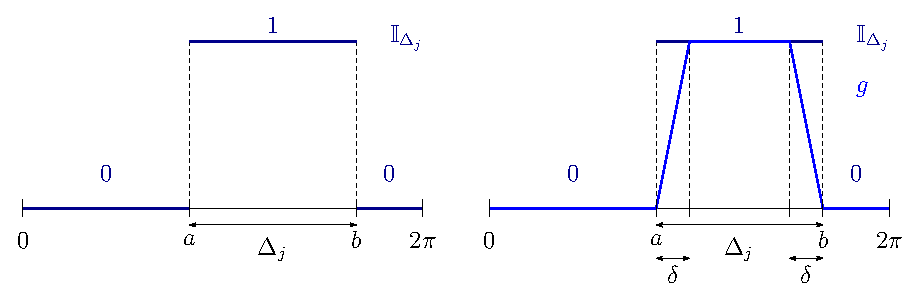
\includegraphics[width=0.85\textwidth]{MA3L27_4.eps}
			\label{MA3L27_4}
			\caption{Построение непрерывной функции из функции индикатора на $[0,2\pi]$.}
			\label{fig: Построение функции}
		\end{figure}
		$$
			g_j(x) = 
			\left\{
			\begin{array}{rl}
				0, & x \in [0,2\pi] \setminus \left[a , b \right] \\[10pt]
				\dfrac{x - a}{\delta}, & x \in  \left[a , a + \delta \right]\\[10pt]
				1, & x \in  \left[a + \delta, b - \delta \right]\\[10pt]
				\dfrac{b - x}{\delta}, & x \in  \left[b - \delta , b  \right]
			\end{array}
			\right. \Rightarrow 			g_j(x) = 
			\left\{
			\begin{array}{rl}
				0, & x \in \MR \setminus \displaystyle \bigsqcup\limits_{k \in \MZ}\left[a + 2\pi k, b + 2\pi k\right] \\[10pt]
				\dfrac{x - a}{\delta}, & x \in  \left[a + 2\pi k, a + \delta + 2\pi k\right], \, \forall k \in \MZ \\[10pt]
				1, & x \in  \left[a + \delta + 2\pi k, b - \delta + 2\pi k\right], \, \forall k \in \MZ \\[10pt]
				\dfrac{b - x}{\delta}, & x \in  \left[b - \delta + 2\pi k, b +  2\pi k\right], \, \forall k \in \MZ
			\end{array}
			\right.
		$$
		Посмотрим, будет ли $\MTI_{\Delta_j}(x)$ приближаться функцией $g_j(x)$ с точки зрения сходимости по норме:
		$$
			\ddint{0}{2\pi}|\MTI_{\Delta_j}(x) - g_j(x)|^2dx = \ddint{a}{a+\delta}|\MTI_{\Delta_j}(x) - g_j(x)|^2dx + \ddint{b - \delta}{b}|\MTI_{\Delta_j}(x) - g_j(x)|^2dx \leq \ddint{a}{a+\delta}dx + \ddint{b - \delta}{b}dx = 2\delta
		$$
		Таким образом, выбирая $\delta$ достаточно маленьким, мы получим любую точность. Пусть каждую индикаторную функцию $\MTI_{\Delta_j}(x)$ мы научились приближать соответствующей функцией $g_j(x)$ для любого промежутка $\Delta_j, \, j = \overline{1,N}$ внутри $[0,2\pi]$:
		$$
			\forall j = \overline{1,N}, \, \forall \VE > 0, \, \exists \, \delta > 0 \colon \delta < \dfrac{\VE^2}{2} \Rightarrow
			\sqrt{\ddint{0}{2\pi}\left|\MTI_{\Delta_j}(x) - g_j(x)\right|^2dx } < \sqrt{2\delta} < \VE
		$$
		Рассмотрим произвольную линейную комбинацию индикаторных функций и оценим её разность с линейной комбинацией приближающих функций:
		$$
			\left\|\ddsum{j = 1}{N}c_j\MTI_{\Delta_j} - \ddsum{j = 1}{N}c_j g_j\right\| \leq \ddsum{j = 1}{N}|c_j|{\cdot}\left\|\MTI_{\Delta_j} - g_j\right\| \leq \left(\ddsum{j = 1}{N}|c_j|\right)\VE 
		$$
		В силу произвольности $\VE>0$, можно сделать эту оценку сколь угодно маленькой:
		$$
			\forall \VE > 0, \, \exists \, \delta > 0 \colon \delta <  \dfrac{\VE^2}{2\left(\sum\limits_{j = 1}^{N}|c_j| + 1\right)^2} \Rightarrow \left\|\ddsum{j = 1}{N}c_j\MTI_{\Delta_j} - \ddsum{j = 1}{N}c_j g_j\right\| < \VE
		$$
		\setcounter{enumi}{0}
		\item Приблизим интегрируемую функцию линейной комбинацией индикаторов. Разобьем отрезок $[0,2\pi]$ на полуинтервалы разбиением $\MTB$: $\Delta_k = [x_{k-1}, x_k)$, $\Delta_N = [x_{N-1},x_N]$. Возьмем функцию:
		$$
			f_{\MTB}(x) = \ddsum{k = 1}{N}\inf\limits_{\Delta_k}f{\cdot}\MTI_{\Delta_k}(x)
		$$
		по сути это нижняя сумму Дарбу. Следовательно, мы хотим показать следующее:
		$$
			\lim\limits_{\lambda(\MTB) \to 0}\ddint{0}{2\pi}|f(x) - f_{\MTB}(x)|^2 dx = 0
		$$
		Функция $f$ - интегрируема на $[0,2\pi] \Rightarrow$ ограничена, пусть $M = \sup\limits_{[0,2\pi]}|f|$, оценим интеграл:
		$$
			\ddint{0}{2\pi}|f(x) - f_{\MTB}(x)|^2 dx \leq 2M\ddint{0}{2\pi}|f(x) - f_{\MTB}(x)|dx = 2M\ddsum{k = 1}{N}\ddint{x_{k-1}}{x_k}\left|f(x) - \inf\limits_{\Delta_k}f\right|dx \leq
		$$
		$$
			\leq 2M\ddsum{k = 1}{N}\ddint{x_{k-1}}{x_k}\left(\sup\limits_{\Delta_k}f - \inf\limits_{\Delta_k}f\right)dx = 2M\ddsum{k = 1}{N}\omega(f,\Delta_k){\cdot}(x_{k} - x_{k-1}) 
		$$
		где $\omega(f,\Delta_k) = \sup\limits_{\Delta_k}f - \inf\limits_{\Delta_k}f$ (см. утверждение $4$, лекцию $17$, семестр $1$). Таким образом, мы получили разность верхней и нижней суммы Дарбу, следовательно по критерию Дарбу (см. теорему $1$, лекцию $24$, семестр $2$ или там же критерий интегрируемости):
		$$
			2M\ddsum{k = 1}{N}\omega(f,\Delta_k){\cdot}(x_{k} - x_{k-1}) = 2M (S(f,\MTB) - s(f,\MTB)) \xrightarrow[\lambda(\MTB)]{} \overline{\MI} - \underline{\MI} = 0
		$$
	\end{enumerate}
	Следовательно, можем подвести итог:
	$$
		\|f - T_P\| \leq \|f - f_{\MTB}\| + \left\|f_{\MTB} - \ddsum{k=1}{N}\inf\limits_{\Delta_k}f{\cdot}g_k\right\| + \left\|\ddsum{k=1}{N}\inf\limits_{\Delta_k}f{\cdot}g_k - T_P\right\|
	$$
	Как мы только что показали:
	$$
		\forall \VE > 0, \, \exists \, \hat{\delta} > 0 \colon \forall (\MTB,\xi), \, \lambda(\MTB) < \hat{\delta} \Rightarrow \|f - f_{\MTB}\| < \VE
	$$
	$$
		\forall \VE > 0, \, \exists \, g_k(x) \in C(\MR), \, g_k(x + 2\pi) = g_k(x), \, k = \overline{1,N} \colon \left\|f_{\MTB} - \ddsum{k=1}{N}\inf\limits_{\Delta_k}f{\cdot}g_k\right\| < \VE
	$$
	$$
		\forall \VE > 0, \, \exists \, P_0 \colon \forall P > P_0, \, \sup\limits_{x \in [0,2\pi]}\left\|\ddsum{k=1}{N}\inf\limits_{\Delta_k}f{\cdot}g_k - T_P\right\| < \VE
	$$
	Таким образом, выберем некоторое $\VE > 0$, найдем $\hat{\delta} > 0$ такое, что наша функция $f(x)$ приближается линейной комбинацией индикаторных функций, то есть фиксируем разбиение $\MTB$. Для индикаторов найдутся $2\pi$-периодические, непрерывные функции $\Rightarrow$ линейная комбинация также будет $2\pi$-периодической и непрерывной $\Rightarrow$ для заранее заданного $\VE$ найдем $P$ при котором $T_P(x)$ будет конечной линейной комбинацией нашей о.н.с., тогда:
	$$
		\forall f \in R[0,2\pi], \, \forall \VE > 0, \, \exists \, T_P \colon \|f - T_P\| \leq 3\VE
	$$
	А это есть ничто иное, как свойство полноты.
\end{proof}
\begin{corollary}
	$\forall f \in R[0,2\pi]$ раскладывается в ряд Фурье по системе: $
	\left\{\dfrac{1}{\sqrt{2\pi}}, \, \dfrac{\cos{nx}}{\sqrt{\pi}}, \, \dfrac{\sin{nx}}{\sqrt{\pi}}  \biggm\vert  n \in \MN  \right\}
	$.
\end{corollary}
Посмотрим как устроены коэффициенты Фурье в таком разложении:
$$
	\inner{f}{\dfrac{1}{\sqrt{2\pi}}} = \ddint{0}{2\pi}f(x)\dfrac{1}{\sqrt{2\pi}}dx = \dfrac{1}{\sqrt{2\pi}}\ddint{0}{2\pi}f(x)dx
$$
$$
	\inner{f}{ \dfrac{\cos{nx}}{\sqrt{\pi}}} = \dfrac{1}{\sqrt{2\pi}}\ddint{0}{2\pi}f(x)\cos{(nx)}dx, \,
	\inner{f}{ \dfrac{\sin{nx}}{\sqrt{\pi}}} = \dfrac{1}{\sqrt{2\pi}}\ddint{0}{2\pi}f(x)\sin{(nx)}dx
$$
Тем самым, ряд Фурье будет иметь следующий вид:
$$
	\inner{f}{\dfrac{1}{\sqrt{2\pi}}}{\cdot}\dfrac{1}{\sqrt{2\pi}} + \ddsum{n = 1}{\infty}\left(\inner{f}{ \dfrac{\cos{nx}}{\sqrt{\pi}}}{\cdot}\dfrac{\cos{nx}}{\sqrt{\pi}} + \inner{f}{ \dfrac{\sin{nx}}{\sqrt{\pi}}}{\cdot}\dfrac{\sin{nx}}{\sqrt{\pi}}\right)
$$
Исторически принято записывать его иначе. Рассмотрим слагаемые ряда по отдельности:
$$
	\inner{f}{ \dfrac{\cos{nx}}{\sqrt{\pi}}}{\cdot}\dfrac{\cos{nx}}{\sqrt{\pi}} = \dfrac{1}{\pi}\ddint{0}{2\pi}f(t)\cos{(nt)}dt{\cdot}\cos{(nx)}
$$
аналогично будет для синуса. Поэтому тригонометрический ряд Фурье приобретет вид:
$$
	\dfrac{a_0}{2} + \ddsum{n = 1}{\infty}\left(a_n \cos{(nx)} + b_n \sin{(nx)}\right)
$$
$$
	a_n = \dfrac{1}{\pi}\ddint{0}{2\pi}f(t)\cos{(nt)}dt, \, \forall n \in \MN
$$
$$	
	b_n = \dfrac{1}{\pi}\ddint{0}{2\pi}f(t)\sin{(nt)}dt, \, \forall n \in \MN
$$
В результате, $\forall f \in R[0,2\pi]$ будет верно:
$$
	\sqrt{\ddint{0}{2\pi} \left|f(x) -   \left(\dfrac{a_0}{2} + \ddsum{n = 1}{N}\left(a_n \cos{(nx)} + b_n \sin{(nx)}\right)\right) \right|^2 dx}  \xrightarrow[N \to \infty]{} 0 \eqno{(*)}
$$
Заметим, что равенство функции ряду Фурье не является поточечным равенством:
$$
	f(x) = \dfrac{a_0}{2} + \ddsum{n = 1}{\infty}\left(a_n \cos{(nx)} + b_n \sin{(nx)}\right)  \eqno{(**)}
$$
Это равенство надо понимать в смысле сходимости выше, то есть: $(*) \Leftrightarrow (**)$. Например, можно представить, что $(*)$ не изменится, если мы изменим значение функции $f$ в одной точке. И как мы уже отмечали ранее, стремление интеграла к нулю не  означает, что подинтегральные функции стремятся к нулю, более того подинтегральная функция может не стремиться к нулю ни в одной точке (см. например пример Рисса, лекция $12$). 
\begin{rem}
	Такая сходимость называется \uwave{среднеквадратической сходимостью}. Как только что заметили, из неё не следует сходимости почти всюду (дополнительно отметим, что из поточечной сходимости следует сходимость почти всюду).
\end{rem}

 Поэтому возникает вопрос, когда будет выполнено поточечное равенство? 
\end{document}